\subsection{Controller}

\begin{figure}[htbp]
   \centering
   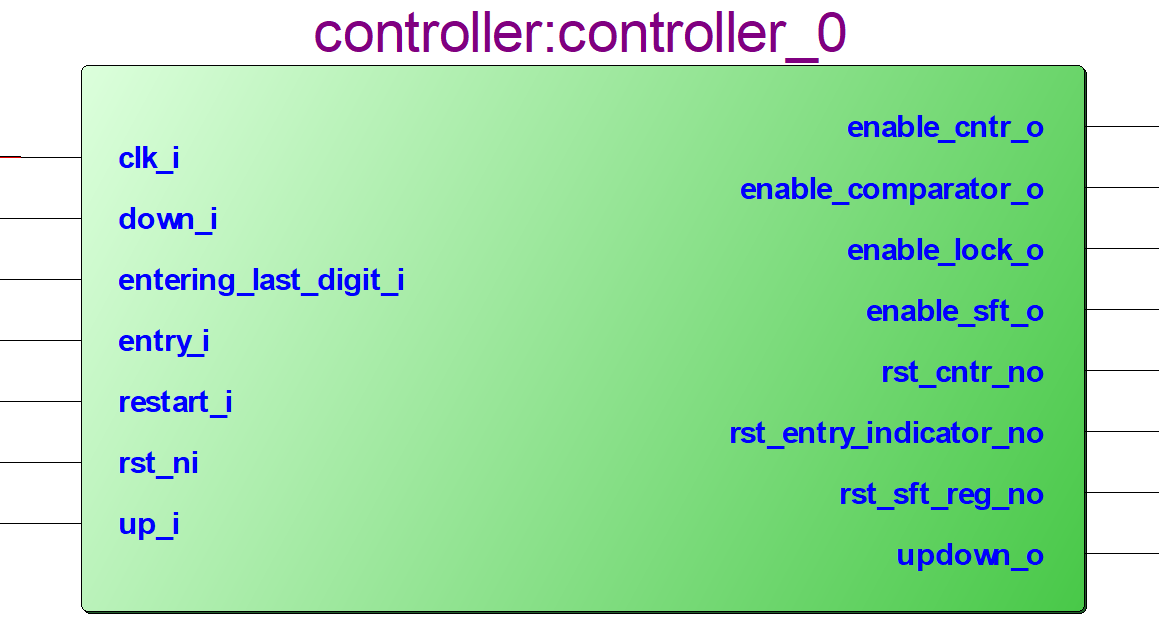
\includegraphics[width=0.85\textwidth]{controller_block_diagram.png}
   \caption{Block diagram of the controller module.}
   \label{fig:controller_block_diagram}
\end{figure}

The controller is a finite state machine which takes key presses and a reset switch as inputs, and outputs enable signals and flag signals to the downstream modules. Fig.~\ref{fig:controller_block_diagram} is the block diagram of the controller, and Fig.~\ref{fig:controller_asm} is the controller's ASM chart. The controller has three states: Idle, Entering, and Entered. In Idle state, the system will not respond to any input except restart signal. In Entering state, the controller will output signals and flags to manipulate the counter and shift register based on the inputs. In Entered state, the controller will disable counter and shift register and enable comparator and lock. When controller is reset, its state goes back to Idle. When controller is restarted, its state goes to Entering.

\begin{figure}[htbp]
   \centering
   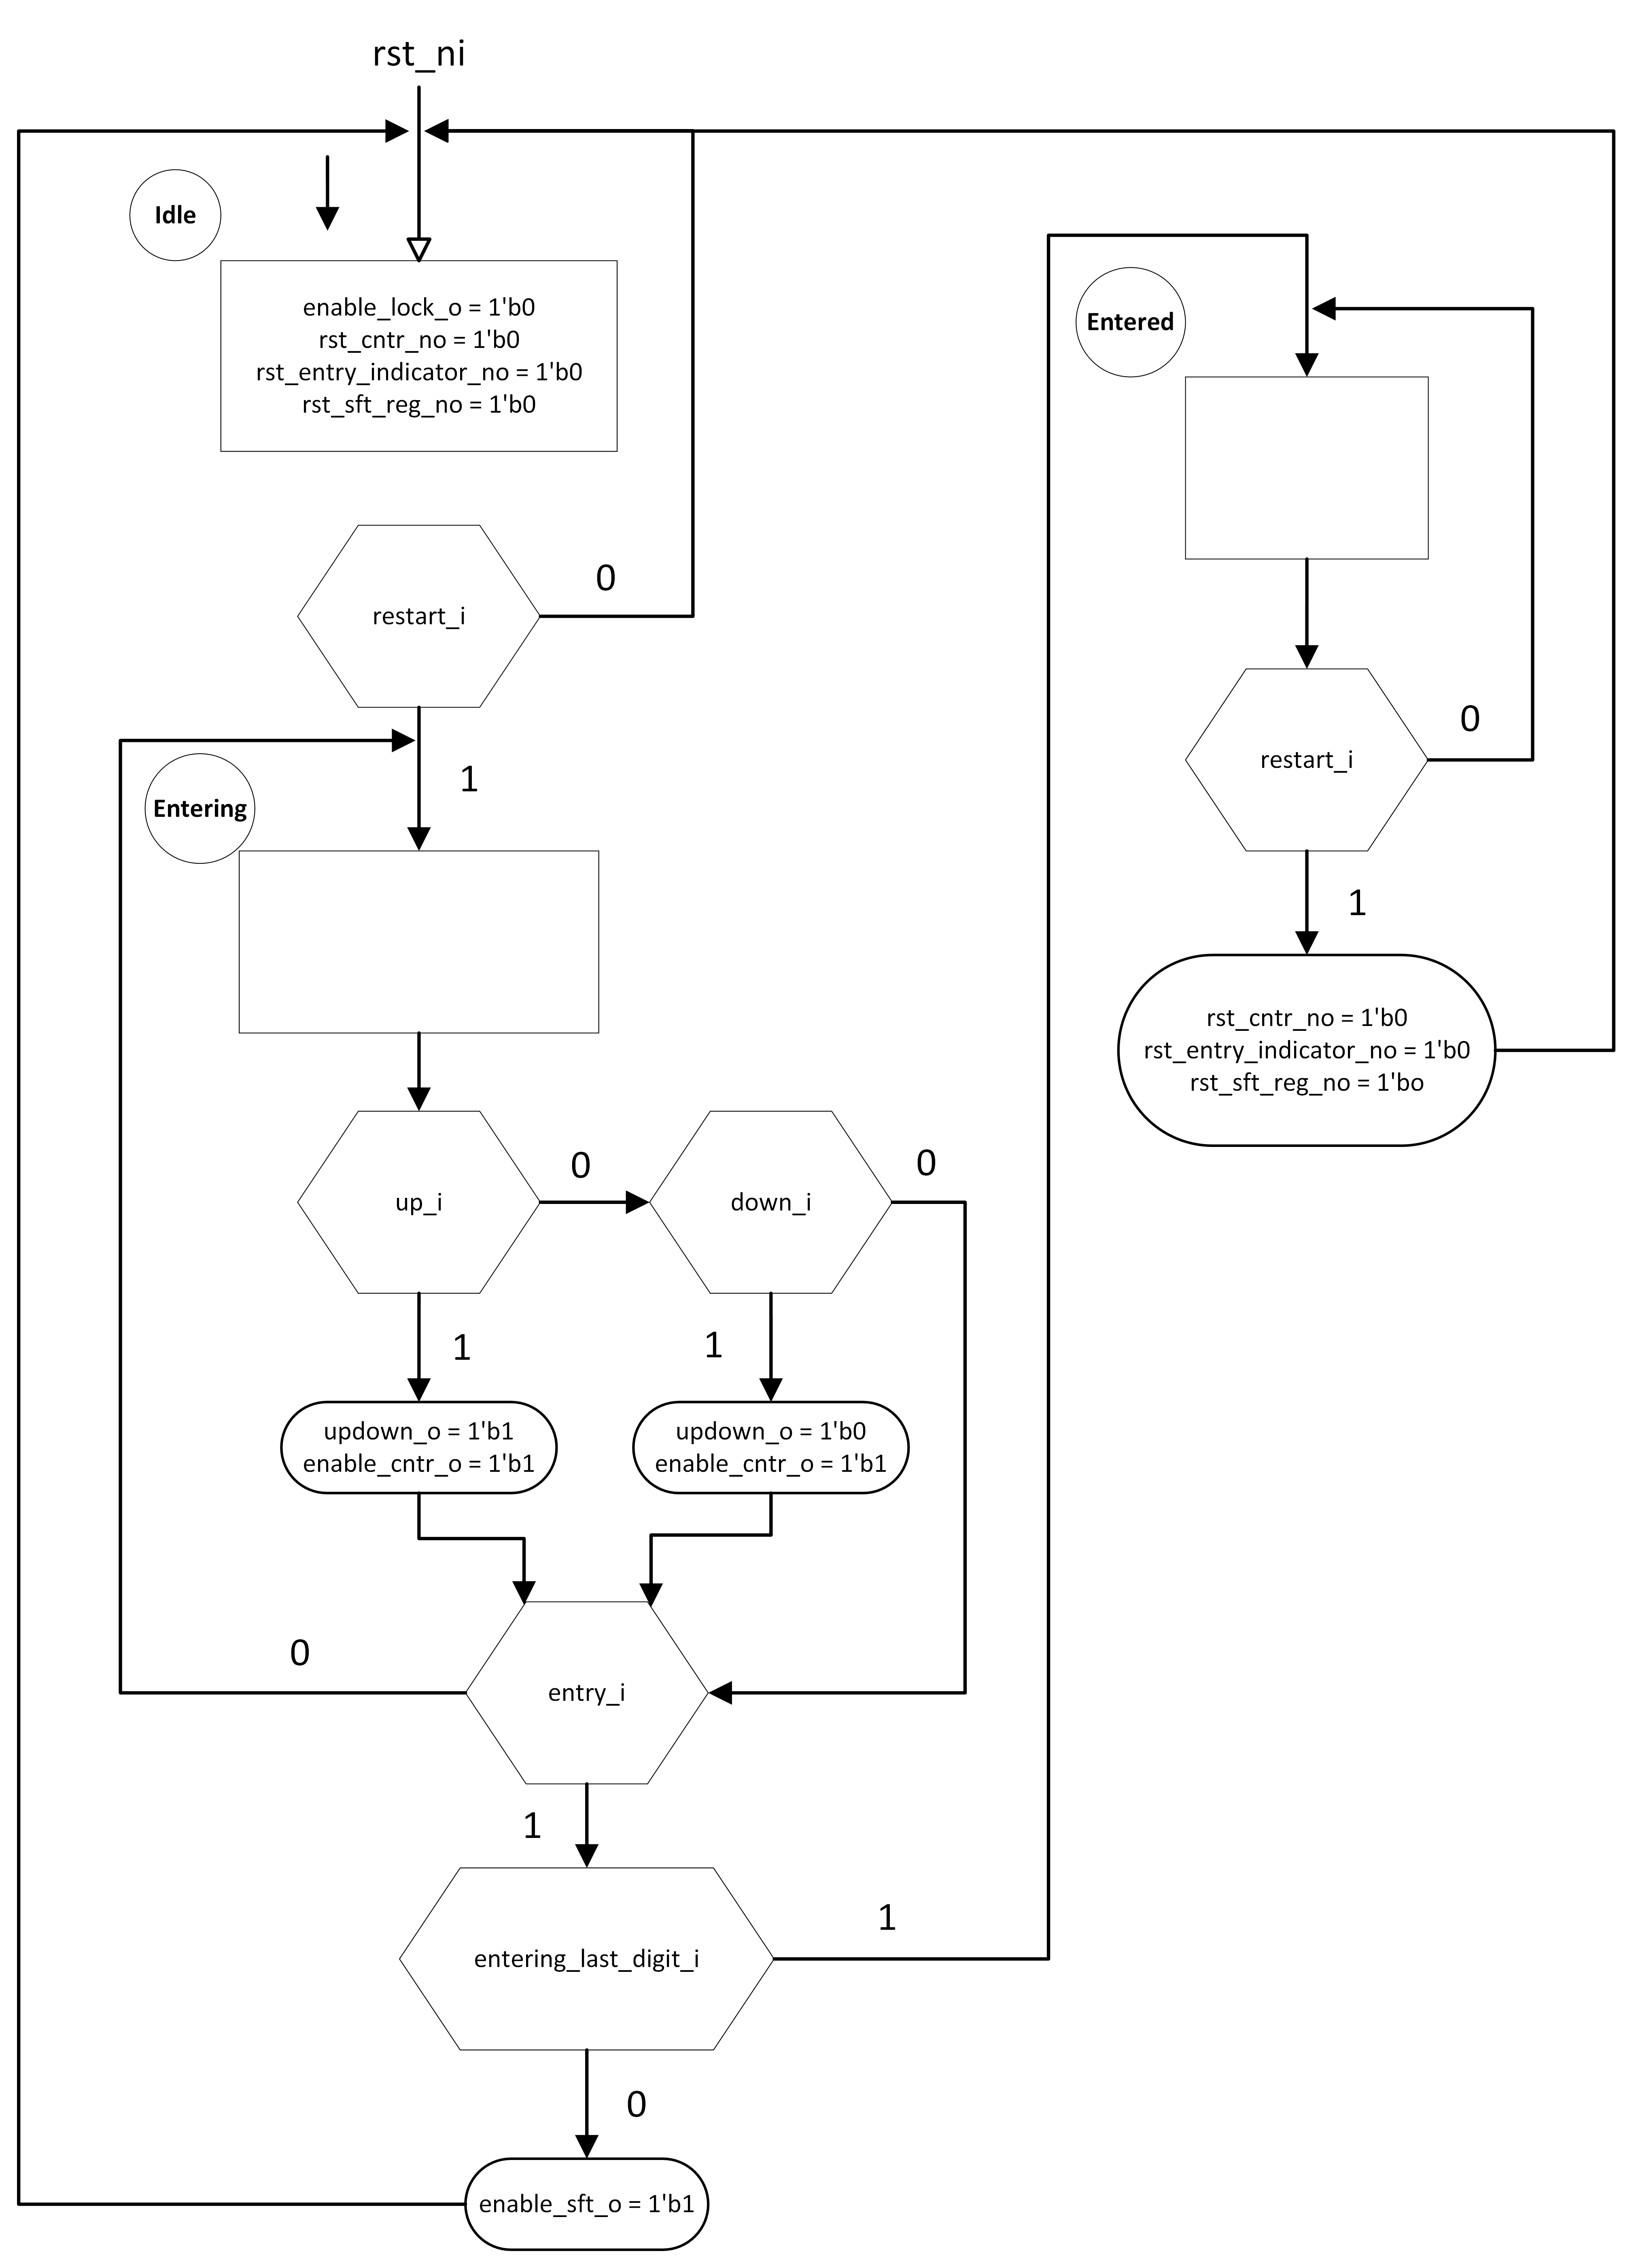
\includegraphics[width=0.85\textwidth]{controller_asm.png}
   \caption{ASM chart of the controller module.}
   \label{fig:controller_asm}
\end{figure}

\begin{minted}[
   fontsize=\footnotesize,
   linenos,
   breaklines,
]{verilog}
module controller (  // glue logic
   input clk_i,
   input rst_ni,
   input up_i,
   input down_i,
   input entry_i,
   input restart_i,
   input entering_last_digit_i,
   output reg enable_cntr_o,
   output reg updown_o,
   output reg enable_sft_o,
   output reg enable_lock_o,
   output reg rst_cntr_no,
   output reg rst_entry_indicator_no,
   output reg rst_sft_reg_no
);

reg [1:0] state_d, state_q;
parameter Idle = 2'b00;
parameter Entering = 2'b01;
parameter Entered  = 2'b10;

always @(posedge clk_i, negedge rst_ni)
   if (~rst_ni)
      state_q <= Idle;
   else
      state_q <= state_d;

always @(state_q, up_i, down_i, entry_i, restart_i) begin
   state_d = state_q;
   enable_cntr_o = 1'b0;
   updown_o = 1'b1;
   enable_sft_o = 1'b0;
   enable_lock_o = 1'b1;
   rst_cntr_no = 1'b1;
   rst_entry_indicator_no = 1'b1;
   rst_sft_reg_no = 1'b1;

   case (state_d)
      Idle: begin
         enable_lock_o = 1'b0;
         rst_cntr_no = 1'b0;
         rst_entry_indicator_no = 1'b0;
         rst_sft_reg_no = 1'b0;
         if (restart_i)
            state_d = Entering;
      end

      Entering: begin
         if (up_i) begin
            updown_o = 1'b1;
            enable_cntr_o = 1'b1;
         end else if (down_i) begin
            updown_o = 1'b0;
            enable_cntr_o = 1'b1;
         end

         if (entry_i)
            if (entering_last_digit_i)
               state_d = Entered;
            else
               enable_sft_o = 1'b1;
      end

      Entered:
         if (restart_i) begin
            state_d = Entering;
            rst_cntr_no = 1'b0;
            rst_entry_indicator_no = 1'b0;
            rst_sft_reg_no = 1'b0;
         end
   endcase
end

endmodule
\end{minted}

\begin{minted}[
   fontsize=\footnotesize,
   linenos,
   breaklines,
]{verilog}
module controller_tb;

// Inputs
reg clk;
reg rst_n;
reg up_i;
reg down_i;
reg entry_i;
reg restart_i;
reg entering_last_digit_i;

// Outputs
wire enable_cntr_o;
wire updown_o;
wire enable_sft_o;
wire enable_lock_o;
wire rst_cntr_no;
wire rst_entry_indicator_no;
wire rst_sft_reg_no;

controller DUT (
   .clk_i(clk),
   .rst_ni(rst_n),
   .up_i(up_i),
   .down_i(down_i),
   .entry_i(entry_i),
   .restart_i(restart_i),
   .entering_last_digit_i(entering_last_digit_i),
   .enable_cntr_o(enable_cntr_o),
   .updown_o(updown_o),
   .enable_sft_o(enable_sft_o),
   .enable_lock_o(enable_lock_o),
   .rst_cntr_no(rst_cntr_no),
   .rst_entry_indicator_no(rst_entry_indicator_no),
   .rst_sft_reg_no(rst_sft_reg_no)
);

// Create a 50Mhz clock
always #10 clk = !clk;  // every ten nanoseconds invert

initial begin
   clk = 1'b0;  // at time 0
   rst_n = 1'b0;  // reset is active
   up_i = 1'b0;
   down_i = 1'b0;
   entry_i = 1'b0;
   restart_i = 1'b0;
   entering_last_digit_i = 1'b0;
end

initial begin
   #20 rst_n = 1'b1;  // release reset

// State: Idle

   // Move to State Entering
   @(posedge clk);
   restart_i = 1'b1;
   @(posedge clk);
   restart_i = 1'b0;

// State: Entering

   @(posedge clk);
   up_i = 1'b1;
   @(posedge clk);
   up_i = 1'b0;

   @(posedge clk);
   down_i = 1'b1;
   @(posedge clk);
   down_i = 1'b0;

   @(posedge clk);
   entry_i = 1'b1;
   @(posedge clk);
   entry_i = 1'b0;

   // Move to State Entered
   entering_last_digit_i = 1'b1;
   @(posedge clk);
   entry_i = 1'b1;
   @(posedge clk);
   entry_i = 1'b0;

// State: Entered

   @(posedge clk);
   up_i = 1'b1;
   @(posedge clk);
   up_i = 1'b0;

   @(posedge clk);
   down_i = 1'b1;
   @(posedge clk);
   down_i = 1'b0;

   @(posedge clk);
   entry_i = 1'b1;
   @(posedge clk);
   entry_i = 1'b0;

   // Move to State Entering
   @(posedge clk);
   restart_i = 1'b1;
   @(posedge clk);
   restart_i = 1'b0;
   entering_last_digit_i = 1'b0;

// State: Entering

   @(posedge clk);
   up_i = 1'b1;
   @(posedge clk);
   up_i = 1'b0;

   @(posedge clk);
   down_i = 1'b1;
   @(posedge clk);
   down_i = 1'b0;

   @(posedge clk);
   entry_i = 1'b1;
   @(posedge clk);
   entry_i = 1'b0;

// Reset

   #20 rst_n = 1'b0;

// Finish the Simulation
   #100;
   $finish;
end

endmodule
\end{minted}

\begin{figure}[htbp]
   \centerline{
   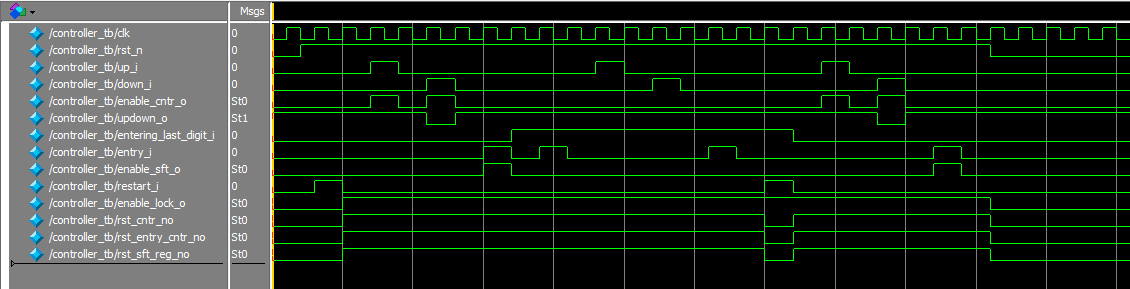
\includegraphics[width=\paperwidth]{controller_sim.png}}
   \caption{Testbench simulation of the controller module.}
   \label{fig:controller_sim}
\end{figure}

Fig.~\ref{fig:controller_sim} shows the simulation test results of the counter module. After reset was released, the controller was in the Idle state. Pressing the restart key under Idle state relased the reset of the counter, entry indicator, and shift register, enabled the lock, and entered the Entering state. In Entering state, up and down pulse triggered enable counter signal. The down pulse also put the updown signal in low voltage level for one clock cycle. The entry pulse enabled the shift register so that the digits stored in it were shifted once. Inputting entry when flag signal, entering last digit, was raised brought the controller into the Entered state. In Entered state, up, down, and entry had no effect, except the restart reset counter, entry indicator, and shift register and brought the controller into the Entering state.
